\documentclass[12pt,a4paper]{report}

\usepackage[a4paper, margin=1in]{geometry}
\geometry{margin=1in}
\usepackage{titlesec}
\usepackage{listings}
\usepackage{algorithm}
\usepackage{algpseudocode}
\usepackage{dirtytalk}
\usepackage{graphicx}
\usepackage{amsmath}
\usepackage{hyperref}
\usepackage{setspace}
\usepackage{lmodern}
\usepackage[utf8]{inputenc}
\usepackage[T1]{fontenc}

\lstset{
  basicstyle=\ttfamily\small,
  keywordstyle=\bfseries\color{blue},
  commentstyle=\itshape\color{gray},
  stringstyle=\color{red},
  numbers=left,
  numberstyle=\tiny,
  frame=single,
  tabsize=2,
  captionpos=b,
  breaklines=true,
  showstringspaces=false,
  aboveskip=0.5em,        % less space above
  belowskip=0.5em,        % less space below
  lineskip=-1pt,          % tighter lines
  xleftmargin=0.5em,
  xrightmargin=0.5em
}
\onehalfspacing
\begin{document}

\tableofcontents
\newpage
\section{Methodology}

\subsection{Pre-processing}
\subsection{Map-Matching}
After the data has been processed, it needs to be matched to a route that exists in reality. The best way to do this is to "snap" the gpx path to a network of roads from OpenStreetMap.
Paul Newson and John Krumm (2016) have developed a method to doing this using Hidden Markov Matching.
Formally, they define a sequence of GPS measurements, $z_t$, but for the purpose of this paper, we shall call observations.
In the segmentation program, the input GPX file will supply the observations in the form of track points.
An observation series can be defined as:
\\
\[
	\mathcal{O}[t] = \{o_1,o_2,\dots,o_T\}, \quad \text{where} o_t = \{(lat_t,long_t,t)\}
\]

A road network can be defined as $\mathcal{G} = (\mathcal{V}, \mathcal{E})$, with nodes $\mathcal{V}$ and edges $\mathcal{E}$. The goal of Newson and Krumm
was to find the most probable sequence of roads that forms a path $\mathcal{P}$ through network $\mathcal{G}$ that matches observations $\mathcal{O}$.
Newson and Krumm explore four different methods of finding $\mathcal{P}$:
\begin{itemize}
	\item Geometric Model
	\item Topological Model
	\item Probabilistic Model (What they focus on)
	\item Kalman Filters
\end{itemize}
The Probabilistic model formalizes map-matching as a \textbf{maximum-likelyhood estimation} problem, using a Hidden Markov Model (HMM).
The paper states the definition of a HMM:\\
\say{The HMM models processes that involve a path through many
	possible states, where some state transitions are more likely than
	others and where the state measurements are uncertain}\\
The algorithm proposed takes individual road sections, and maps them onto the states of the HMM. It then will attempt to "match each location measurement
with the proper road segment".  This means that every GPX track point will be mapped to a road segment object.
To find the appropriate road section, each observation is matched with several possible roads that it could snap to, and the most probable path is
selected.\\
In order to find the most probable route, Newson and Krumm introduce the concept of Emission Probabilities (EPs). These give the likelyhood that "a measurement occurs from a specific state."
In the context of map-matching, each road-observation pair has an EP measurement:
\[
	p(o_t \;| \mathcal{E}_i)
\]
where:
\begin{itemize}
	- $o_t$ is the observation at time $t$,
	- $\mathcal{E}_i$ is the $i^{th}$ road segment (of our network of edges, $\mathcal{G}$).
\end{itemize}
Intuitively, road segments further from the observation are less likely to match than closer ones.
Formally, there exists a point on each road section, $x_{t,i}$, that is the closest point to $o_t$.
The paper uses a Great Circle closest point approach, which is implemented in the Haversine formula.
We define this as:
\[
	||o_t - x_{t,i}||_{\textit{haversine}}
\]

In reality, any value greater than the width of the road is due to GPS noise. GPS noise has been described as a \textit{zero-mean Gaussian} model by Frank van Diggelen (2007).
This leads to the implementation of $p$:
\[
	p(o_t \;| \mathcal{E}_i) = \frac{1}{\sqrt{2\pi}\sigma_o}e^{0.5\bigg(\frac{\left\|o_t - x_{t,i}\right\|_{\textit{haversine}}}{\sigma_o}\bigg)^2}
\]
where $\sigma_o$ is the standard deviation of GPS observations.\\
This represents the confidence in the observation GPS data.
In the paper, a maximum distance is set at 200m, so that any road that's closest point is further than 200m away is automatically discarded to reduce the candidate quantity.

The most important point of the paper is how it is determined which road the next observation is on. To do this, a conventional route planner plots the road distance between
two points, $x_{t,i}$ and $x_{t+1,j}$, on road candidates $\mathcal{E}_i$ and $\mathcal{E}_j$ respectively, denoted as $\left\|x_{t,i} - x_{t+1,j}\right\|_{\textit{route}}$. Empirically, the distance between the two points and distance between two observations
should be about the same, as both distances are very short, and the variance should be small. They calculated a histogram, which fit closely to an exponential probability distribution as seen in the following figure:

\begin{figure}[h!]
	\centering
	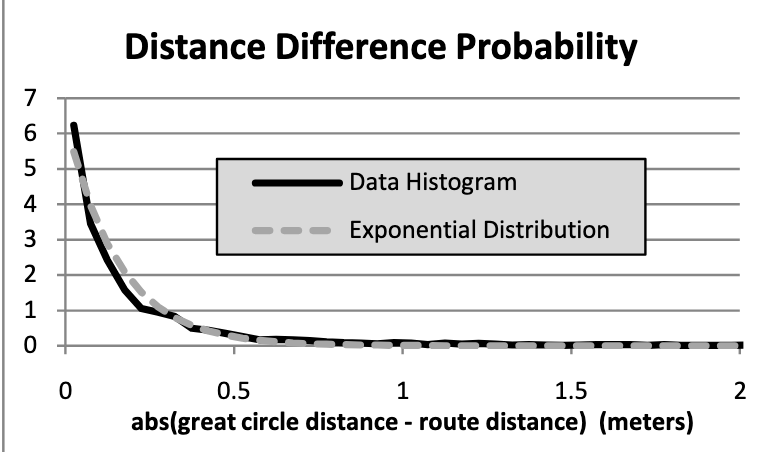
\includegraphics[width=0.7\textwidth]{histogram.png}
	\caption{Histogram courtesy of Paul Newson and John Krumm (2016)}
\end{figure}

The formula that fits the curve is:
\[
	p(d_t) = \frac{1}{\beta}e^{\frac{-d_t}{\beta}}
\]
where:
\[
	d_t = \bigg | \left\|o_t - o_{t-1}\right\|_{\textit{great circle}} - \left\|x_{t,i*} - x_{t+1,j*}\right\|_{\textit{route}}\bigg |
\]
$i*$ and $j*$ are the "ground truth segments", defined as the roads taken in the test drive, and the value $\beta$ is the probability parameter, which represents a tolerance of non-direct routes.
This means a route that has a lot of back roads and detours would require a higher $\beta$ than a cross-country road trip on a highway.

To figure the most optimal path, a Viterbi algorithm determines, through dynamic recursive programming, the most optimal path through the lattice that would
maximize the product of both EP and transition properties. This would then statistically be the most probable route that the observation array follows.
The approach to this is as follows:
\begin{enumerate}
	\item Initialize the algorithm by creating an array \texttt{delta[t, s]} of size $T \times N$, and a backpointer array \texttt{psi} of the same size.
	\item For each value $t$ > 0, and each $s$:
	      \[
		      \texttt{delta[t,s]} = \text{max}_{s'} \bigg(\delta[t-1, s'] \cdot transition[t-1, s', s]\bigg) \cdot emission[t,s]
	      \]
	      Where $max_{s'}$ is the candidate segment that lead to the largest solution of $s'$ at time $t-1$.
	      The value $s'$ that lead to the highest probability of leading to $s$ is stored in \texttt{psi}
	\item Termination of the algorithm occurs when we reach, $s_T$ and use \texttt{psi} to recover the optimal path.
\end{enumerate}

\newpage
The pseudocode for this would look something like:
\begin{lstlisting}
  array o[t] = [list of gpx points]
  array2D candidate_states[t,S] = [every candidate road object S for each $o_t$]
  array2D emission[t, s] = [emission probability matrix, P($o_t | s$)]
  array2D transition[s, s'] = [transition probability matrix, P(s_curr, s_prev)]
  array init[s] = [initial state probabilities (P($s_0$))]
  
  # initialize delta and psi
  for each s in $s_0$
  delta[0, s] = init[s] * emission[0,s])
  psi[0, s] = null

  #Recursively calculate path
  T = sizeof(o) - 1
  for t from (1,T):
    for each s in candidate_states:
      max_prob = 0
      best_prev = null
      # get previous state probabilities
      for each s' in candidate_states[t-1, s]:
        prob = delta[t-1, s'] * transition[s', s] * emission[t, s]
        if prob > max_prob:
          max_prob = prob
          best_prev = s'
      delta[t,s] = max_prob
      psi[t,s] = best_prev

  #terminate algorithm
  max_final_prob = 0
  last_state = null
  for each s in candidate_states:
    if delta[T,s] > max_final_prob:
      max_final_prob = delta[T,s]
      last_state = s
    
  path[t] = [empty array of size T+1]
  path[T] = last_state
  for t from (T-1, 1):
  path[t] = psi[t+1, path[t+1]]

  return path

\end{lstlisting}


\subsection{Segmentation}
\subsection{Categorization}
\subsection{Segment Analysis}
\subsubsection{Wavelet Transform}
Sharifzadeh et al. (2005) propose the use of the Wavelet Transform Function, and more specifically Wavelet Footprints,
to address the problem of change detection in time series data.
\begin{itemize}
	\item \textbf{Wavelet Decomposition of Trajectory}: \\ Given a signal $x[n]$ of length $N$, it can be expressed as a wavelet series:
	      \[
		      x[n] =
		      \sum_{j=0}^{J-1} \sum_{k} d_{j,k} \, \psi_{j,k}[n]
		      + \sum_{k} c_{J,k} \, \phi_{J,k}[n]
	      \]
	      where:
	      \begin{itemize}
		      \item $\psi_{j,k}[n]$ are the wavelet basis functions at scale $j$ and position $k$.
		      \item $\phi_{J,k}[n]$ are the scaling functions at the coarsest level $J$.
		      \item $d_{j,k}$ are detail coefficients at scale $j$ and position $k$.
		      \item $c_{J,k}$ are approximation coefficients.
	      \end{itemize}
	\item \textbf{Footprint Definition}\\
	      The \textbf{wavelet footprint} of $x$ is defined as the set of significant coefficients:
	      \[
		      F(x) = \{ (j,k) \;|\; |d_{j,k}| > T_j \}
	      \]
	      where $T_j$ is a scale-dependent threshold, which can be tuned to correspond to physiological thresholds of training intensity zones. This is useful since
	      at different scales, the detail coefficients are not comparable, so the threshold must be defined explicitly.

	\item \textbf{Footprint Calculation}\\
	      To calculate the Wavelet Footprint, first the detail coefficient, $d_{j,k}$ is extracted. Since not all detail coefficients are meaningful, a scale-dependent threshold $T_j$
	      is defined to filter out noise. This is calculated with the standard deviation of the specific scale:
	      \[
		      T_j = \gamma_j \dot \sigma_j
	      \]

	      Where:
	      \begin{itemize}
		      \item $\sigma_j$ is the standard deviation of $d_{j,k}$ at scale $j$.
		      \item $\gamma_j$ is the tuning parameter.
	      \end{itemize}
	      This value can then be used to define the Footprint Definition described earlier.

	\item \textbf{Compact Representation}\\
	      To reduce dimensionality, only the $k$ largest coefficients can be retained:
	      \[
		      F_k(x) = \text{top-}k \text{ elements of } F(x)
	      \]
	      This is useful to optimize data set size, while not reducing the accuracy of the data significantly.
	\item \textbf{Matching and Distance}\\
	      The overall difference in two signals $x$ and $y$ can be approximated by taking the difference of their footprints:
	      \[
		      D(x,y) \approx \| F(x) - F(y) \|
	      \]

\end{itemize}
\subsubsection{Normalized Power}
Applying Normalized Power is a useful metric for determining variability in power data. The longer the signal, the more useful NP would be, so
we can apply a weighting inversely proportional to the average duration of the segment.
However, as the time gets shorter, we can mitigate the accuracy loss by tapering off the 30 second rolling average towards the end of the segment.
\\
Instead of a 30 second rolling average, we will take the lesser of either 30 seconds, or the remaining duration of the segment, so we don't end up
with a lot of segments with skewed NP due to the rolling window running off the edge of the data set.\\

We will define a variable $k$ that represents this:
\[
	k[t] = \begin{cases}
		(T-t), & (T-t) < 30   \\
		30,    & (T-t) \ge 30 \\
	\end{cases}
\]
Now we can define the rolling average, ${P}_{r}$ at time $t$ to be:
\[
	\overline{P}_{r}[t] = \frac{1}{k[t]} \sum_{j=0}^{k[t]-1} P[j]
\]
The final definition of NP is:
\[
	\mathrm{NP} = \bigg( \frac{1}{M} \sum_{i=1}^{M}\big(\overline{P}_{r}[i]\big)^{4}\bigg)^{1/4}
\]


\subsection{Training Suitability Score Evaluation}
\end{document}
